\subsection{Comparing Clustering Results: Hungarian Algorithm}

Since we tried different clustering methods, it would be vital to come
up with a statistics to compare different clustering
results. Essentially, there should be two steps in this procedure. \\

\noindent Let say we are going to compare two clustering results, $C$
and $C^{'}$, each containing $n$ clusters, i.e. $c_1, c_2, ... c_n$
and $c^{'}_1, c^{'}_2, ... c^{'}_n$.\\

\noindent First step is to determine an one to one mapping
$$f: \{c_i: i=1...n\} \rightarrow \{c^{'}_i: i=1...n\}$$

\noindent Given a mapping $f$, we can compute the Rand Index for the
two clustering results, which is a typical measure of the similarity
between two data clusterings.\\

\noindent We are supposed to find a mapping $f$ to maximize the
similarity (Rand Index), and take the maximal Rand Index as a
similarity measure of the two clustering results, as described by
Hungarian Algorithm\cite{hungarian} (The Hungarian method is a combinatorial
optimization algorithm that solves the assignment problem in
polynomial time and which anticipated later primal-dual methods. It
was developed and published in 1955 by Harold Kuhn, who gave the name
``Hungarian method'' because the algorithm was largely based on the
earlier works of two Hungarian mathematicians).


\subsection{Finding Critical Questions dominating clustering Results}

Here we intend to figure out which of those questions are most
critical forclustering. To be consistent, here we always perform k-means
clustering on original data aggregated over county. We set the k-means
results of the whole dataset as ``standard clustering''.\\

\noindent To see how important a question is, we remove the
corresponding column for that question from the original dataset, and
then apply k-means clustering on the new dataset. After that, using
the method mentioned previously, we compute a similarity measure
between this clustering results and the ``standard clustering''. We
perform this procedure ten times on each of the 67 questions and take the average similarity measure (k-means is not perfectly stable), as shown in
Figure~\ref{fig:removeQuestion}.\\


\begin{figure}
\centering
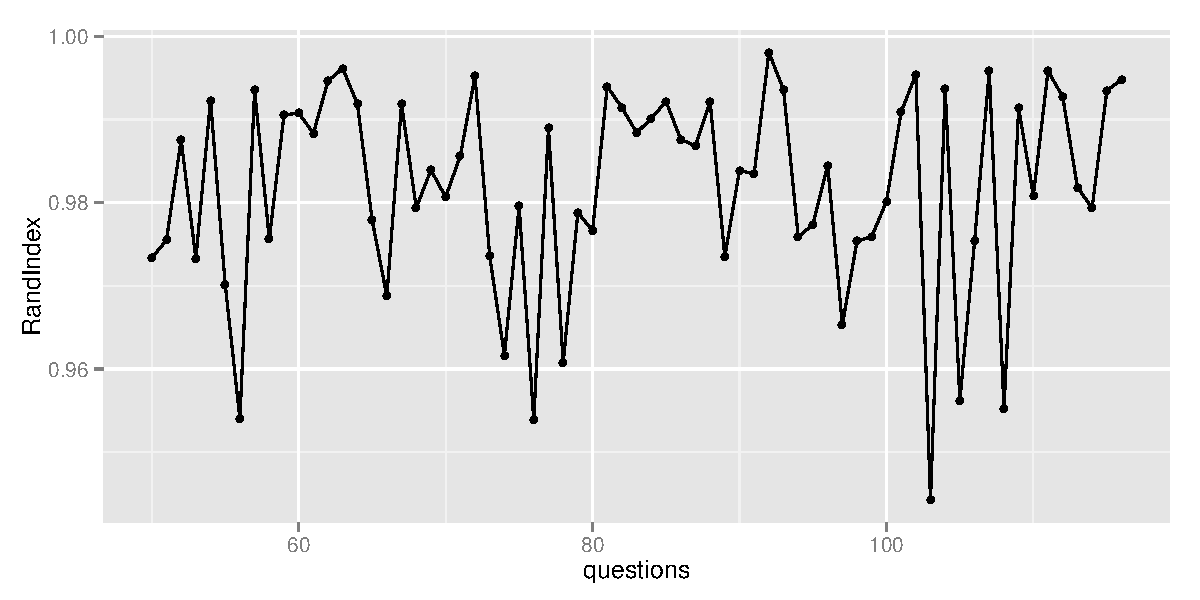
\includegraphics[width=0.9\linewidth]{fig/remove-question-clustering-difference.pdf}
\caption{remove-question-clustering-difference} \label{fig:removeQuestion}
\end{figure}

\noindent As we can see from Figure xx, clearly there are 5 questions
perturbing the clustering results significantly, which are question
56, 76, 103, 105, 108. From the Dialect Survey website, we have these
four questions as follow:

\begin{itemize}

\item Q056: Pantyhose are so expensive anymore that I just try to get
a good suntan and forget about it.

\item Q076: What term do you use to refer to something that is across
both streets from you at an intersection (or diagonally across from
you in general)?

\item Q103: What do you call the thing from which you might drink
water in a school?

\item Q105: What is your generic term for a sweetened carbonated
beverage?

\item Q108: What vowel do you use in bag?


\end{itemize}

\noindent We are lucky to pick out Q076 in section 2 by visually
selection. The plots for the answer of each of these four questions
can be found in our \textbf{Shiny} app.
